% Options for packages loaded elsewhere
\PassOptionsToPackage{unicode}{hyperref}
\PassOptionsToPackage{hyphens}{url}
%
\documentclass[
  letterpaper,
  ignorenonframetext,
  aspectratio=43,
  handout,
  12pt]{beamer}
\usepackage{pgfpages}
\setbeamertemplate{caption}[numbered]
\setbeamertemplate{caption label separator}{: }
\setbeamercolor{caption name}{fg=normal text.fg}
\beamertemplatenavigationsymbolsempty
% Prevent slide breaks in the middle of a paragraph
\widowpenalties 1 10000
\raggedbottom
\setbeamertemplate{part page}{
  \centering
  \begin{beamercolorbox}[sep=16pt,center]{part title}
    \usebeamerfont{part title}\insertpart\par
  \end{beamercolorbox}
}
\setbeamertemplate{section page}{
  \centering
  \begin{beamercolorbox}[sep=12pt,center]{part title}
    \usebeamerfont{section title}\insertsection\par
  \end{beamercolorbox}
}
\setbeamertemplate{subsection page}{
  \centering
  \begin{beamercolorbox}[sep=8pt,center]{part title}
    \usebeamerfont{subsection title}\insertsubsection\par
  \end{beamercolorbox}
}
\AtBeginPart{
  \frame{\partpage}
}
\AtBeginSection{
  \ifbibliography
  \else
    \frame{\sectionpage}
  \fi
}
\AtBeginSubsection{
  \frame{\subsectionpage}
}
\usepackage{amsmath,amssymb}
\usepackage{lmodern}
\usepackage{ifxetex,ifluatex}
\ifnum 0\ifxetex 1\fi\ifluatex 1\fi=0 % if pdftex
  \usepackage[T1]{fontenc}
  \usepackage[utf8]{inputenc}
  \usepackage{textcomp} % provide euro and other symbols
\else % if luatex or xetex
  \usepackage{unicode-math}
  \defaultfontfeatures{Scale=MatchLowercase}
  \defaultfontfeatures[\rmfamily]{Ligatures=TeX,Scale=1}
\fi
\usetheme[]{metropolis}
% Use upquote if available, for straight quotes in verbatim environments
\IfFileExists{upquote.sty}{\usepackage{upquote}}{}
\IfFileExists{microtype.sty}{% use microtype if available
  \usepackage[]{microtype}
  \UseMicrotypeSet[protrusion]{basicmath} % disable protrusion for tt fonts
}{}
\makeatletter
\@ifundefined{KOMAClassName}{% if non-KOMA class
  \IfFileExists{parskip.sty}{%
    \usepackage{parskip}
  }{% else
    \setlength{\parindent}{0pt}
    \setlength{\parskip}{6pt plus 2pt minus 1pt}}
}{% if KOMA class
  \KOMAoptions{parskip=half}}
\makeatother
\usepackage{xcolor}
\IfFileExists{xurl.sty}{\usepackage{xurl}}{} % add URL line breaks if available
\IfFileExists{bookmark.sty}{\usepackage{bookmark}}{\usepackage{hyperref}}
\hypersetup{
  hidelinks,
  pdfcreator={LaTeX via pandoc}}
\urlstyle{same} % disable monospaced font for URLs
\newif\ifbibliography
\usepackage{longtable,booktabs,array}
\usepackage{calc} % for calculating minipage widths
\usepackage{caption}
% Make caption package work with longtable
\makeatletter
\def\fnum@table{\tablename~\thetable}
\makeatother
\usepackage{graphicx}
\makeatletter
\def\maxwidth{\ifdim\Gin@nat@width>\linewidth\linewidth\else\Gin@nat@width\fi}
\def\maxheight{\ifdim\Gin@nat@height>\textheight\textheight\else\Gin@nat@height\fi}
\makeatother
% Scale images if necessary, so that they will not overflow the page
% margins by default, and it is still possible to overwrite the defaults
% using explicit options in \includegraphics[width, height, ...]{}
\setkeys{Gin}{width=\maxwidth,height=\maxheight,keepaspectratio}
% Set default figure placement to htbp
\makeatletter
\def\fps@figure{htbp}
\makeatother
% Make links footnotes instead of hotlinks:
\DeclareRobustCommand{\href}[2]{#2\footnote{\url{#1}}}
\setlength{\emergencystretch}{3em} % prevent overfull lines
\providecommand{\tightlist}{%
  \setlength{\itemsep}{0pt}\setlength{\parskip}{0pt}}
\setcounter{secnumdepth}{-\maxdimen} % remove section numbering
\usepackage{pgfpages}
\pgfpagesuselayout{2 on 1}
\providecommand{\tightlist}{%
\setlength{\itemsep}{0pt}\setlength{\parskip}{0pt}}
\makeatletter
\makeatother
\let\Oldincludegraphics\includegraphics
\renewcommand{\includegraphics}[2][]{\Oldincludegraphics[width=\textwidth,height=0.7\textheight,keepaspectratio]{#2}}
\ifluatex
  \usepackage{selnolig}  % disable illegal ligatures
\fi

\author{}
\date{}

\begin{document}

\begin{frame}{AE 737: Mechanics of Damage Tolerance}
\protect\hypertarget{ae-737-mechanics-of-damage-tolerance}{}
Lecture 16 - Strain based fatigue

Dr.~Nicholas Smith

Wichita State University, Department of Aerospace Engineering

29 March, 2021
\end{frame}

\begin{frame}{schedule}
\protect\hypertarget{schedule}{}
\begin{itemize}
\tightlist
\item
  29 Mar - Strain-based Fatigue
\item
  31 Mar - Crack Growth
\item
  2 Apr - Homework 6 Due
\item
  5 Apr - Boeing Method
\item
  7 Apr - Cycle counting
\item
  9 Apr - Homework 6 Self-grade, Homework 7 Due
\end{itemize}
\end{frame}

\begin{frame}{outline}
\protect\hypertarget{outline}{}
\begin{itemize}
\tightlist
\item
  strain based fatigue
\item
  variable amplitude strains
\item
  mean stress effects
\item
  general trends
\item
  notches
\item
  multiaxial loading
\item
  other factors affecting fatigue
\end{itemize}
\end{frame}

\hypertarget{strain-based-fatigue}{%
\section{strain based fatigue}\label{strain-based-fatigue}}

\begin{frame}{strain based fatigue}
\protect\hypertarget{strain-based-fatigue-1}{}
\begin{itemize}
\tightlist
\item
  The strain based fatigue method uses local stresses and strains
  (instead of global, nominal values)
\item
  The strain-based method gives greater detail, and validity at lower
  cycles
\item
  It is still valid for high cycle fatigue (but gives same result as
  stress-based fatigue)
\item
  Does not include crack growth analysis or fracture mechanics
\end{itemize}
\end{frame}

\begin{frame}{strain life curve}
\protect\hypertarget{strain-life-curve}{}
\begin{itemize}
\tightlist
\item
  Similar to the S-N curves in stress-based fatigue analysis, we can
  plot the cyclic strain amplitude vs.~number of cycles to failure
\item
  This is most commonly done using axial test machines (instead of
  rotating bending tests)
\item
  The test is run in strain control (not load control)
\item
  Generally plotted on log-log scale
\end{itemize}
\end{frame}

\begin{frame}{plastic and elastic strain}
\protect\hypertarget{plastic-and-elastic-strain}{}
\begin{itemize}
\tightlist
\item
  We can separate the total strain into elastic and plastic components
  \[ \epsilon_a = \epsilon_{ea} + \epsilon_{pa}\]
\end{itemize}
\end{frame}

\begin{frame}{plastic strain}
\protect\hypertarget{plastic-strain}{}
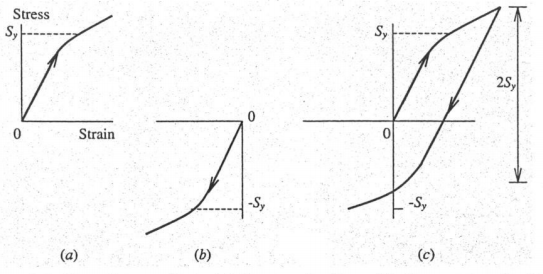
\includegraphics{../images/plastic_strain.PNG}
\end{frame}

\begin{frame}{hysteresis loops}
\protect\hypertarget{hysteresis-loops}{}
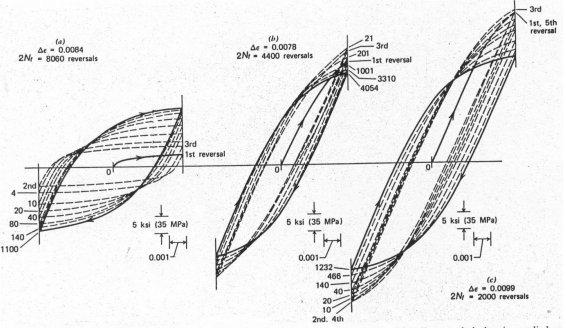
\includegraphics{../images/hysteresis_loops.PNG}
\end{frame}

\begin{frame}{cyclic stress strain curve}
\protect\hypertarget{cyclic-stress-strain-curve}{}
\begin{itemize}
\tightlist
\item
  While strain-life data will generally just report \(\epsilon_a\) and
  \(\epsilon_{pa}\) some will also tabulate a form for the cyclic
  stress-strain curve
\end{itemize}

\[\epsilon_a = \frac{\sigma_a}{E} + \left(\frac{\sigma_a}{H^\prime}\right)^{\frac{1}{n^\prime}}\]
\end{frame}

\begin{frame}{plastic and elastic strain}
\protect\hypertarget{plastic-and-elastic-strain-1}{}
\begin{itemize}
\tightlist
\item
  On strain life curves, the strain is often plotted three times per
  each experiment
\item
  Once for total strain, once for plastic strain, and once for elastic
  strain
\item
  Since plastic strain and elastic strain vary by the number of cycles,
  a hysteresis loop from half the fatigue life is generally used
\item
  This is considered representative of stable behavior
\end{itemize}
\end{frame}

\begin{frame}{experimental data}
\protect\hypertarget{experimental-data}{}
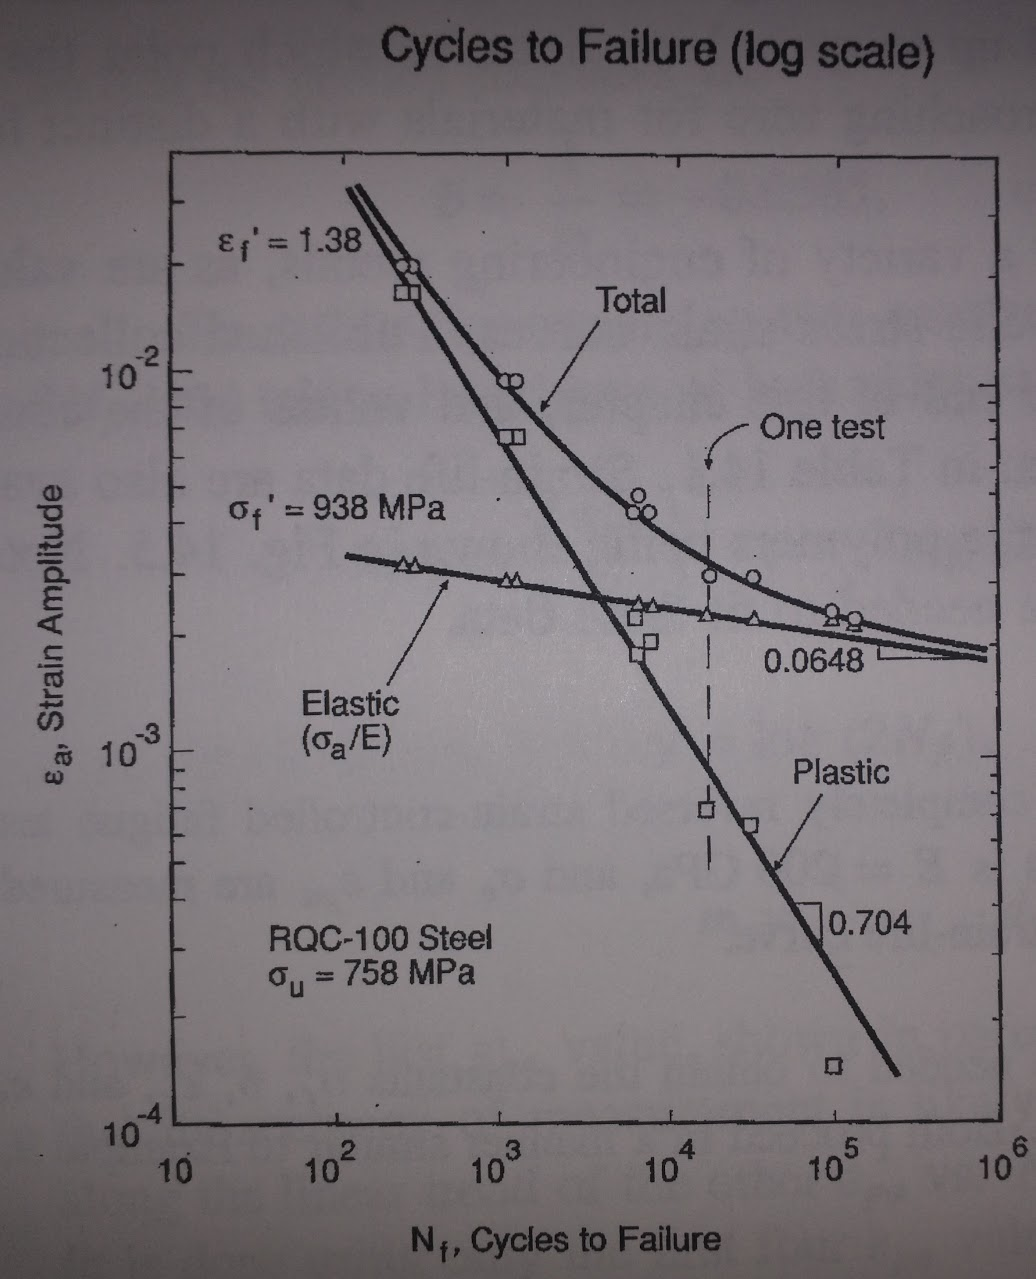
\includegraphics{../images/strain-life.jpg}
\end{frame}

\begin{frame}{trends}
\protect\hypertarget{trends}{}
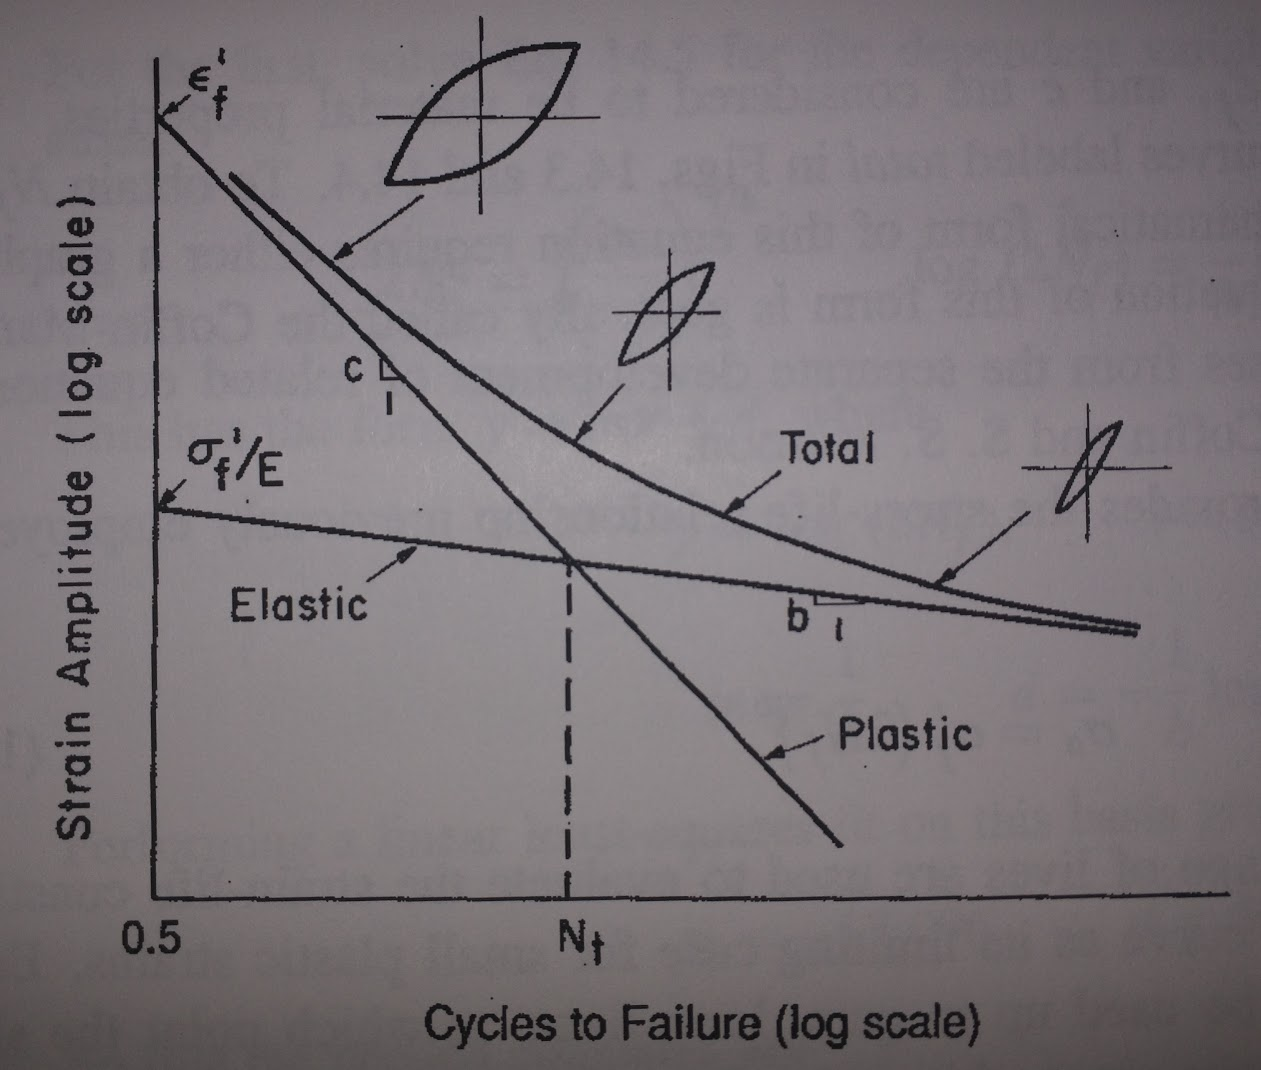
\includegraphics{../images/elastic-plastic.jpg}
\end{frame}

\begin{frame}{lines}
\protect\hypertarget{lines}{}
\begin{itemize}
\tightlist
\item
  We notice that the data for elastic and plastic strains are
  represented by straight lines, in the log-log scale
\item
  If we recall the form used for a straight line in log-log plots for
  S-N curves:
\end{itemize}

\[ \sigma_a = \sigma_f^\prime (2 N_f)^b\]

\begin{itemize}
\tightlist
\item
  We can convert this to find the elastic component of strain
\end{itemize}

\[\epsilon_{ea} = \frac{\sigma_f^\prime}{E} (2N_f)^b\]
\end{frame}

\begin{frame}{lines}
\protect\hypertarget{lines-1}{}
\begin{itemize}
\tightlist
\item
  We can use the same form with new constants for the plastic component
  of strain
\end{itemize}

\[ \epsilon_{pa} = \epsilon_f^\prime (2 N_f)^c\]

\begin{itemize}
\tightlist
\item
  We can combine the elastic and plastic portions to find the total
  strain-life curve
\end{itemize}

\[\epsilon_a = \frac{\sigma_f^\prime}{E} (2N_f)^b + \epsilon_f^\prime (2 N_f)^c\]
\end{frame}

\begin{frame}{example}
\protect\hypertarget{example}{}
\begin{longtable}[]{@{}cccr@{}}
\toprule
\(\epsilon_a\) & \(\sigma_a\) (MPa) & \(\epsilon_{pa}\) &
\(N_f\) \\ \addlinespace
\midrule
\endhead
0.0202 & 631 & 0.01695 & 227 \\ \addlinespace
0.0100 & 574 & 0.00705 & 1030 \\ \addlinespace
0.0045 & 505 & 0.00193 & 6450 \\ \addlinespace
0.0030 & 472 & 0.00064 & 22250 \\ \addlinespace
0.0023 & 455 & (0.00010) & 110000 \\ \addlinespace
\bottomrule
\end{longtable}
\end{frame}

\begin{frame}{transition life}
\protect\hypertarget{transition-life}{}
\begin{itemize}
\tightlist
\item
  With the strain-based fatigue method we are better equipped to discuss
  the difference between high and low-cycle fatigue
\item
  Low-cycle fatigue is dominated by plastic effects, while high-cycle
  fatigue has little plasticity
\item
  We can find the intersection of the plastic strain and elastic strain
  lines
\item
  This point is \emph{N}\emph{t}, the transition fatigue life
\end{itemize}

\[N_t = \frac{1}{2}\left(\frac{\sigma_f^\prime}{\epsilon_f^\prime}\right)^{\frac{1}{c-b}}\]
\end{frame}

\begin{frame}{inconsistencies in constants}
\protect\hypertarget{inconsistencies-in-constants}{}
\begin{itemize}
\tightlist
\item
  If we consider the equation for the cyclic stress train curve
\end{itemize}

\[\epsilon_a = \frac{\sigma_a}{E} + \left(\frac{\sigma_a}{H^\prime}\right)^{\frac{1}{n^\prime}}\]

\begin{itemize}
\tightlist
\item
  We can consider the plastic portion and solve for \(\sigma_a\)
\end{itemize}

\[\sigma_a = H^\prime \epsilon_{pa}^{n^\prime} \]
\end{frame}

\begin{frame}{inconsistencies in constants}
\protect\hypertarget{inconsistencies-in-constants-1}{}
\begin{itemize}
\tightlist
\item
  We can eliminate \(2N_f\) from the plastic strain equation
\end{itemize}

\[ \epsilon_{pa} = \epsilon_f^\prime (2 N_f)^c\]

\begin{itemize}
\tightlist
\item
  By solving the stress-life relationship for \(2 N_f\)
\end{itemize}

\[ \sigma_a = \sigma_f^\prime (2 N_f)^b \]

and substituting that into the plastic strain
\end{frame}

\begin{frame}{inconsistencies in constants}
\protect\hypertarget{inconsistencies-in-constants-2}{}
\begin{itemize}
\tightlist
\item
  We then compare with stress-life equations and find
\end{itemize}

\[\begin{aligned}
 H^\prime &= \frac{\sigma_f^\prime}{(\epsilon_f^\prime)^{b/c}}\\
 n^\prime &= \frac{b}{c}
\end{aligned}\]
\end{frame}

\begin{frame}{inconsistencies in constants}
\protect\hypertarget{inconsistencies-in-constants-3}{}
\begin{itemize}
\tightlist
\item
  However, in practice these constants are fit from different curves
\item
  In some cases there can be large inconsistencies in these values
\item
  One cause for this is data that do not lie on a straight line in the
  log-log domain
\item
  For ductile materials at short lives, the true stresses and strains
  may differ significantly from engineering stress and strain
\end{itemize}
\end{frame}

\hypertarget{variable-amplitude-strains}{%
\section{variable amplitude strains}\label{variable-amplitude-strains}}

\begin{frame}{variable amplitude strains}
\protect\hypertarget{variable-amplitude-strains-1}{}
\begin{itemize}
\tightlist
\item
  As with stresses, we can apply variable amplitude strains
\item
  However, when the change is made will affect whether there is a
  tensile or compressive mean stress
\end{itemize}
\end{frame}

\begin{frame}{compressive mean}
\protect\hypertarget{compressive-mean}{}
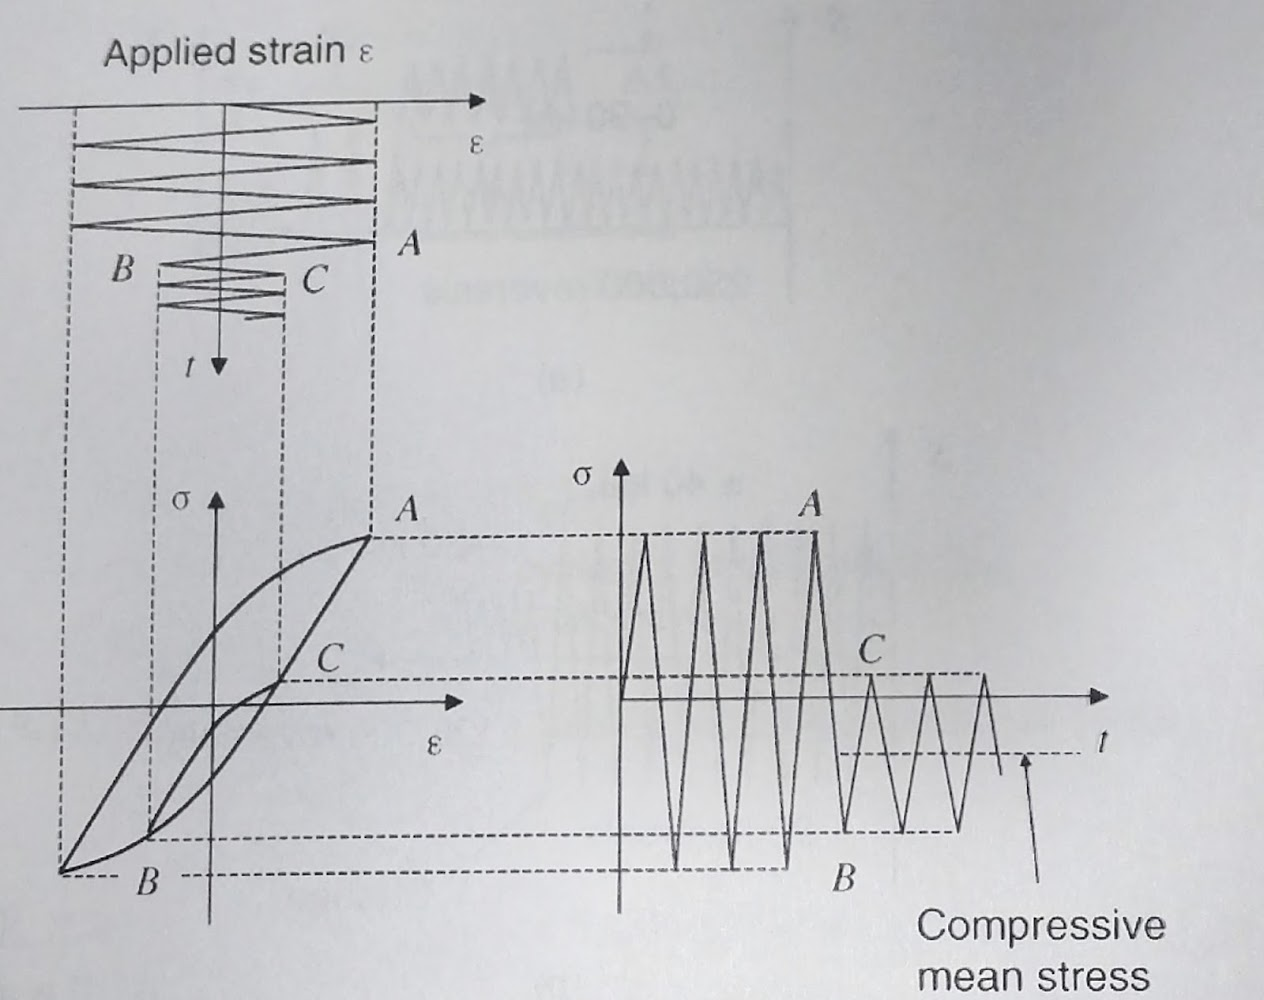
\includegraphics{../images/compressive_mean.jpg}
\end{frame}

\begin{frame}{tensile mean}
\protect\hypertarget{tensile-mean}{}
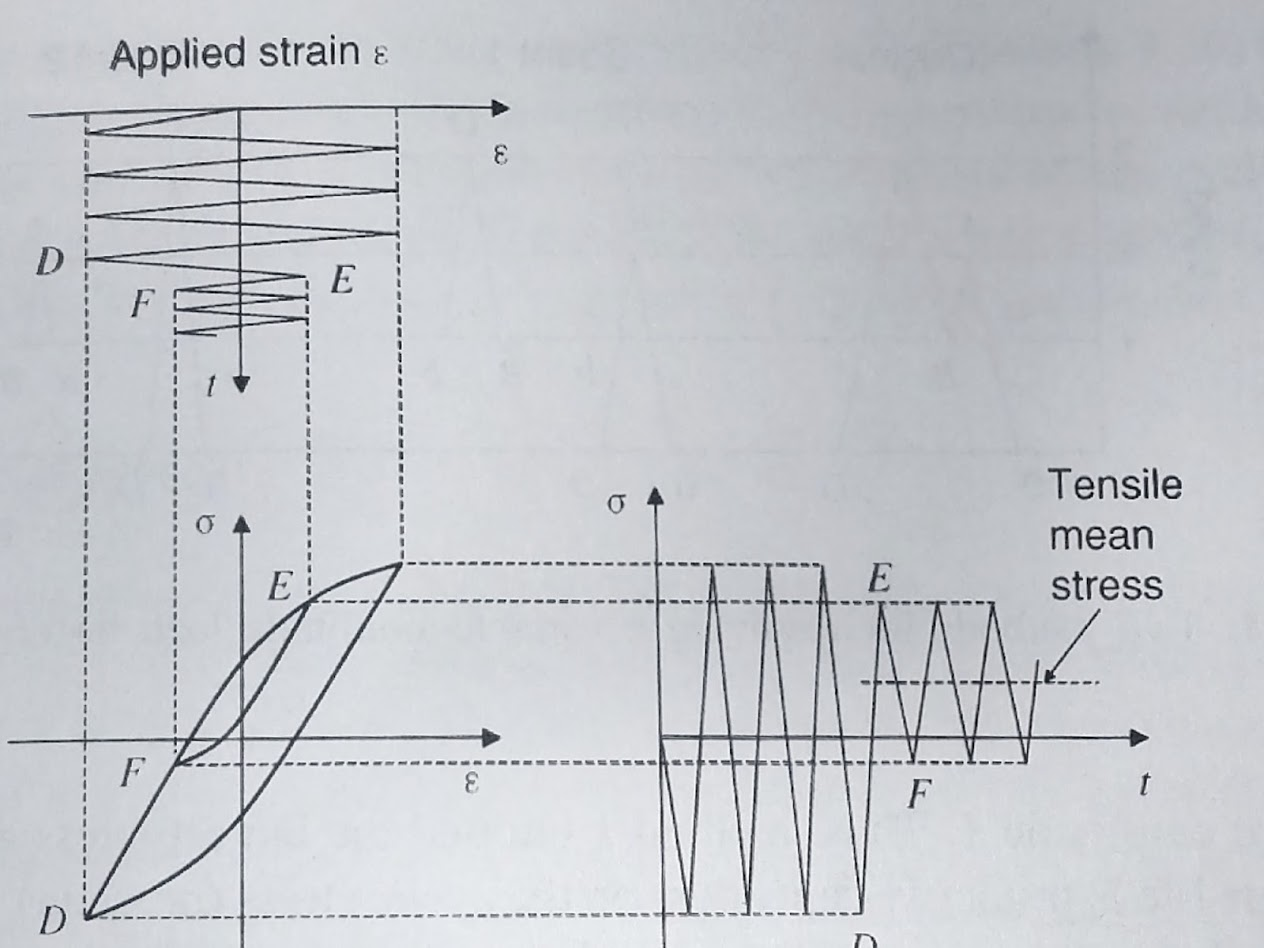
\includegraphics{../images/tensile_mean.jpg}
\end{frame}

\hypertarget{mean-stress-effects}{%
\section{mean stress effects}\label{mean-stress-effects}}

\begin{frame}{mean stress in strain-based fatigue}
\protect\hypertarget{mean-stress-in-strain-based-fatigue}{}
\begin{itemize}
\tightlist
\item
  In regions where plastic strain is significant, some applied mean
  stress is likely to be relaxed through cyclic plastic strain
\item
  When the plastic strain is not significant, mean stress will exist
\item
  Mean strain does not generally affect fatigue life
\end{itemize}
\end{frame}

\begin{frame}{morrow approach}
\protect\hypertarget{morrow-approach}{}
\begin{itemize}
\tightlist
\item
  Recall the Morrow approach for mean stress effects from the
  stress-based method
\end{itemize}

\[\frac{\sigma_a}{\sigma_{ar}} + \frac{\sigma_m}{\sigma_f^\prime} = 1\]

\begin{itemize}
\tightlist
\item
  We can rearrange the equation such that
\end{itemize}

\[\sigma_a = \sigma_f^\prime\left[\left(1-\frac{\sigma_m}{\sigma_f^\prime}\right)^\frac{1}{b}(2N_f)\right]^b\]
\end{frame}

\begin{frame}{morrow approach}
\protect\hypertarget{morrow-approach-1}{}
\begin{itemize}
\tightlist
\item
  If we compare to the stress-life equation
  (\(\sigma_a = \sigma_f^\prime (2N_f)\) we see that we can replace
  \(N_f\) with
\end{itemize}

\[N^* = N_f \left(1-\frac{\sigma_m}{\sigma_f^\prime}\right)^\frac{1}{b}\]

\begin{itemize}
\tightlist
\item
  We can now substitute \(N^*\) for \(N_f\) in the strain-life equation
  to find
\end{itemize}

\[\epsilon_a = \frac{\sigma_f^\prime}{E} \left(1-\frac{\sigma_m}{\sigma_f^\prime}\right)(2N_f)^b + \epsilon_f^\prime\left(1-\frac{\sigma_m}{\sigma_f^\prime}\right)^\frac{c}{b} (2 N_f)^c\]
\end{frame}

\begin{frame}{morrow approach}
\protect\hypertarget{morrow-approach-2}{}
\begin{itemize}
\tightlist
\item
  Graphically, we can use the Morrow approach very easily using only the
  zero-mean stress graph
\item
  From the zero-mean stress graph, find the point corresponding to your
  applied strain
\item
  For a non zero mean stress, this point represents
  \((\epsilon_a, N^*)\), we can now solve for \(N_f\) using the equation
  for \(N^*\)
\end{itemize}
\end{frame}

\begin{frame}[fragile]{modified morrow}
\protect\hypertarget{modified-morrow}{}
\begin{itemize}
\tightlist
\item
  While the Morrow equation agrees very well with many data, some are
  better fit with a modification
\item
  In the modified version, it is assumed that the mean stress has no
  effect on the plastic term
\end{itemize}

\[\epsilon_a = \frac{\sigma_f^\prime}{E}\left(1-\frac{\sigma_f}{\sigma_f^\prime}\right)(2N_f)^b + \epsilon_f^\prime (2N_f)^c\]

\begin{itemize}
\tightlist
\item
  There is no convenient solution method for this form, and it generally
  must be solved numerically, or plotted with many families of
  \texttt{\textbackslash{}sigma\_m}
\end{itemize}
\end{frame}

\begin{frame}{smith watson topper}
\protect\hypertarget{smith-watson-topper}{}
\begin{itemize}
\tightlist
\item
  The Smith, Watson, and Topper approach assumes that the life for any
  given state is dependent on the product \(\sigma_{max} \epsilon_a\)
\item
  After some manipulation, this gives
\end{itemize}

\[\sigma_{max} \epsilon_a = \frac{\left(\sigma_f^\prime\right)^2}{E}(2N_f)^{2b} + \sigma_f^\prime \epsilon_f^\prime (2N_f)^{b+c}\]

\begin{itemize}
\tightlist
\item
  This method can also be solved graphically if a plot of
  \(\sigma_{max}\epsilon_a\) is made using zero-mean data. All we need
  to do is find the new \(\sigma_{max}\epsilon_a\) point to find a new
  \(N_f\)
\end{itemize}
\end{frame}

\begin{frame}{comparison}
\protect\hypertarget{comparison}{}
\begin{itemize}
\tightlist
\item
  All three methods discussed are in general use
\item
  The Morrow method is very good for steel
\item
  The modified Morrow method gives improved results in many materials
\item
  The SWT approach is very good for general use, but is non-conservative
  with a compressive mean stress
\end{itemize}
\end{frame}

\begin{frame}{example p.~285}
\protect\hypertarget{example-p.-285}{}
\end{frame}

\begin{frame}{cycle counting}
\protect\hypertarget{cycle-counting}{}
\begin{itemize}
\tightlist
\item
  In all fatigue methods (stress, strain, and crack propagation) the way
  we count load cycles can have an effect on our results
\item
  To avoid being non-conservative, we need to always count the largest
  amplitudes first
\item
  We will discuss some specific cycle-counting algorithms during crack
  propagation
\end{itemize}
\end{frame}

\begin{frame}{cycle counting}
\protect\hypertarget{cycle-counting-1}{}
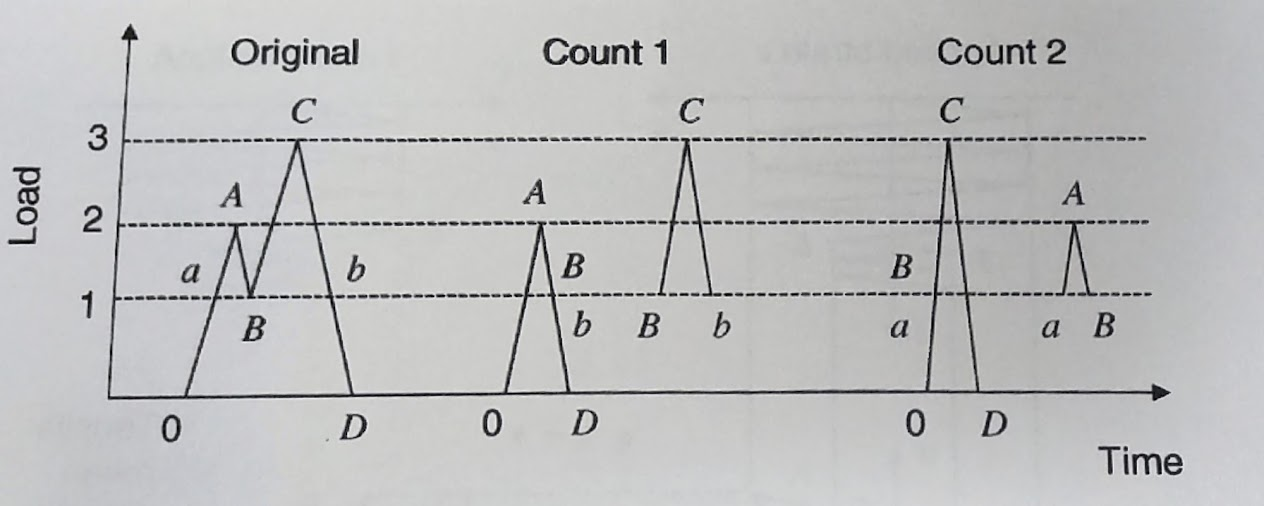
\includegraphics{../images/cycle_counting.jpg}
\end{frame}

\hypertarget{general-trends}{%
\section{general trends}\label{general-trends}}

\begin{frame}{true fracture strength}
\protect\hypertarget{true-fracture-strength}{}
\begin{itemize}
\tightlist
\item
  We can consider a tensile test as a fatigue test with \(N_f = 0.5\)
\item
  We would then expect the true fracture strength
  \(\tilde{\sigma}_f \approx \sigma_f^\prime\)
\item
  And similarly for strain
  \(\tilde{\epsilon}_f \approx \epsilon_f^\prime\)
\end{itemize}
\end{frame}

\begin{frame}[fragile]{ductile materials}
\protect\hypertarget{ductile-materials}{}
\begin{itemize}
\tightlist
\item
  Since ductile materials experience large strains before failure, we
  expect relatively large \(\epsilon_f^\prime\) and relatively small
  \texttt{\textbackslash{}sigma\_f\^{}\textbackslash{}prime}
\item
  This will cause a less steep slope in the plastic strain line
\item
  In turn this intersects with the elastic strain line much later,
  resulting a longer transition life for ductile materials
\end{itemize}
\end{frame}

\begin{frame}{brittle materials}
\protect\hypertarget{brittle-materials}{}
\begin{itemize}
\tightlist
\item
  Brittle materials exhibit the opposite effect, with relatively low
  \(\epsilon_f^\prime\) and relatively high \(\sigma_f^\prime\)
\item
  This results in a steeper plastic strain line
\item
  And shorter transition life
\end{itemize}
\end{frame}

\begin{frame}[fragile]{tough materials}
\protect\hypertarget{tough-materials}{}
\begin{itemize}
\tightlist
\item
  Tough materials have intermediate values for both
  \(\epsilon_f^\prime\) and \(\sigma_f^\prime\)
\item
  This gives a transition life somewhere between brittle and ductile
  materials
\item
  It is also noteworthy that strain-life for many metals pass through
  the point \(\epsilon_a = 0.01\) and \texttt{N\_f\ =\ 1000} cycles
\item
  Steels also follow a trend with Brinell Hardness, the higher they are
  on the HB scale, the lower their transition life
\end{itemize}
\end{frame}

\begin{frame}{typical property ranges}
\protect\hypertarget{typical-property-ranges}{}
\begin{itemize}
\tightlist
\item
  Most common engineering materials have \(-0.8 < c < -0.5\), with most
  values being very close to \emph{c} = -0.6
\item
  The elastic strain slope generally has \emph{b} = -0.085
\item
  A ``steep'' elastic slope is around \emph{b} = -0.12, common in soft
  metals
\item
  While ``shallow'' slopes are around \emph{b} = -0.05, common for
  hardened metals
\end{itemize}
\end{frame}

\hypertarget{notches}{%
\section{notches}\label{notches}}

\begin{frame}{fatigue notch factor}
\protect\hypertarget{fatigue-notch-factor}{}
\begin{itemize}
\tightlist
\item
  We previously found expressions for stress-based fatigue analysis when
  notches are present
\item
  Due to yielding, the notch sensitivity is not the same for stress and
  strain controlled fatigue analysis
\item
  One simple approach to find the strain fatigue notch factor is to use
\end{itemize}

\[K_t = \sqrt{K_f^\sigma K_f^\epsilon}\]
\end{frame}

\hypertarget{multiaxial-loading}{%
\section{multiaxial loading}\label{multiaxial-loading}}

\begin{frame}{multiaxial loading}
\protect\hypertarget{multiaxial-loading-1}{}
\begin{itemize}
\tightlist
\item
  Multi-axial loading in strain-based fatigue analysis is still an
  active field of research
\item
  We are currently only capable of handling proportional loads that are
  in-phase (i.e.~have the same frequency)
\end{itemize}
\end{frame}

\begin{frame}{multiaxial loading}
\protect\hypertarget{multiaxial-loading-2}{}
\begin{itemize}
\tightlist
\item
  If we consider the principal directions where
  \(\sigma_{2a}= \lamba \sigma_{1a}\) we find an expression for the
  strain-life as
\end{itemize}

\[\epsilon_{1a} = \frac{\frac{\sigma_f^\prime}{E}(1-\nu \lambda)(2N_f)^b + \epsilon_f^\prime(1-0.5\lambda)(2N_f)^c}{\sqrt{1-\lambda+\lambda^2}}\]
\end{frame}

\begin{frame}{stress triaxiality factor}
\protect\hypertarget{stress-triaxiality-factor}{}
\begin{itemize}
\tightlist
\item
  Another approach is to consider the stress triaxiality factor
\end{itemize}

\[T = \frac{1+\lambda}{\sqrt{1-\lambda+\lambda^2}}\]

\begin{itemize}
\tightlist
\item
  Three notable cases of this are

  \begin{enumerate}
  \tightlist
  \item
    Pure planar shear: \(\lambda = -1 \qquad T = 0\)
  \item
    Uniaxial stress: \(\lambda = 0 \qquad T = 1\)
  \item
    Equal biaxial stress: \(\lambda = 1 \qquad T = 2\)
  \end{enumerate}
\end{itemize}
\end{frame}

\begin{frame}{stress triaxiality factor}
\protect\hypertarget{stress-triaxiality-factor-1}{}
\begin{itemize}
\tightlist
\item
  Marloff suggests the following inclusion of stress triaxiality
\end{itemize}

\[\bar{\epsilon_a} = \frac{\sigma_f^\prime}{E}(2 N_f)^b + 2^{1-T}\epsilon_f^\prime(2N_f)^c\]
\end{frame}

\hypertarget{other-factors-affecting-fatigue}{%
\section{other factors affecting
fatigue}\label{other-factors-affecting-fatigue}}

\begin{frame}{factors affecting fatigue life}
\protect\hypertarget{factors-affecting-fatigue-life}{}
\begin{itemize}
\tightlist
\item
  At temperatures above one-half the melting temperature (absolute
  scale), creep-relaxation is significant
\item
  This will cause the strain/stress-life curves to become rate dependent
\item
  Occurs at room temperature for many materials (lead, tin, many
  polymers)
\item
  At a sufficiently elevated temperature for any material
\end{itemize}
\end{frame}

\begin{frame}{surface finish}
\protect\hypertarget{surface-finish}{}
\begin{itemize}
\tightlist
\item
  High cycle fatigue is sensitive to surface finish, samples are
  generally polished
\item
  Low cycle fatigue is not sensitive to surface finish or residual
  stress
\item
  The plastic deformation tends to remove residual stresses
\item
  In high-cycle fatigue, crack initiation is important (poor surface
  finish allows cracks to form earlier)
\item
  When plastic deformation is present (low-cycle fatigue), cracks form
  relatively quickly regardless of surface finish
\end{itemize}
\end{frame}

\begin{frame}{surface finish}
\protect\hypertarget{surface-finish-1}{}
\begin{itemize}
\tightlist
\item
  Since low-cycle fatigue has little effect from surface finish, we
  could modify the strain life curve by altering only the elastic
  portion
\item
  If we define the surface effect factor, \(m_s\), we can find a new
  \(b_s\) to replace \emph{b} in the strain-life equation
\end{itemize}

\[b_s = \frac{\log\left(m_s (2N_e)^b\right)}{\log(2N_e)}\]
\end{frame}

\begin{frame}{surface treatments}
\protect\hypertarget{surface-treatments}{}
\begin{itemize}
\tightlist
\item
  Treatments which decrease fatigue life:

  \begin{itemize}
  \tightlist
  \item
    Electro-plating (chrome, +corrosion resistance, -fatigue life)
  \item
    Grinding improves surface finish, but introduces surface tension,
    and heat generated can temper quench
  \item
    Stamping introduces discontinuities and irregularities
  \item
    Forging can refine grain structure and improve physical properties,
    but can cause decarburization in steels, which hurts fatigue life
  \item
    Hot rolling can also cause decarburization
  \end{itemize}
\end{itemize}
\end{frame}

\begin{frame}{surface treatments}
\protect\hypertarget{surface-treatments-1}{}
\begin{itemize}
\tightlist
\item
  Some treatments improve fatigue life:

  \begin{itemize}
  \tightlist
  \item
    Cold rolling improves surface finish, introduces residual
    compressive stress on surface (slows crack initiation on surface)
  \item
    Shot peeing introduces many small divots on surface, which can be
    detrimental in corrosion, but it does cause a residual compressive
    stress on the surface
  \end{itemize}
\end{itemize}
\end{frame}

\begin{frame}{size}
\protect\hypertarget{size}{}
\begin{itemize}
\tightlist
\item
  Size can also have effects on fatigue life
\item
  Larger parts are more susceptible to damage/imperfections at the same
  stress level
\item
  This is why composites are often made from very small fibers (glass
  fiber, carbon fiber, ceramic-matrix composites)
\end{itemize}
\end{frame}

\begin{frame}{size}
\protect\hypertarget{size-1}{}
\begin{itemize}
\tightlist
\item
  The exact effect of size will depend on material, one study for low
  carbon steels found
\end{itemize}

\[m_d = \left(\frac{d}{25.4 \text{mm}}\right)^{-0.093}\]

\begin{itemize}
\tightlist
\item
  Which is then used to re-calculate material constants
\end{itemize}

\[ \sigma_{fd}^\prime = m_d \sigma_f^\prime \qquad \epsilon_{fd}^\prime = m_d \epsilon_f^\prime \]
\end{frame}

\begin{frame}{thermal fatigue}
\protect\hypertarget{thermal-fatigue}{}
\begin{itemize}
\tightlist
\item
  Thermal loading can be introduced when two dissimilar parts are
  attached together, the coefficient of thermal expansion causes them to
  expand differently, introducing extra stresses due to the temperature
  change
\item
  If the temperature is significantly different between two sides of a
  part thermal stresses can also be introduced
\end{itemize}
\end{frame}

\begin{frame}{thermal fatigue}
\protect\hypertarget{thermal-fatigue-1}{}
\begin{itemize}
\tightlist
\item
  Low temperatures generally cause a material to behave in a more
  brittle fashion, which alters the fatigue life
\item
  High temperatures cause problems with creep-relaxation and can also
  affect the crystalline structure
\end{itemize}
\end{frame}

\end{document}
